\documentclass[]{article}
\usepackage{lmodern}
\usepackage{amssymb,amsmath}
\usepackage{ifxetex,ifluatex}
\usepackage{graphicx}
\usepackage[final]{pdfpages}
\usepackage{fixltx2e} % provides \textsubscript
\ifnum 0\ifxetex 1\fi\ifluatex 1\fi=0 % if pdftex
  \usepackage[T1]{fontenc}
  \usepackage[utf8]{inputenc}
\else % if luatex or xelatex
  \ifxetex
    \usepackage{mathspec}
  \else
    \usepackage{fontspec}
  \fi
  \defaultfontfeatures{Ligatures=TeX,Scale=MatchLowercase}
\fi
% use upquote if available, for straight quotes in verbatim environments
\IfFileExists{upquote.sty}{\usepackage{upquote}}{}
% use microtype if available
\IfFileExists{microtype.sty}{%
\usepackage{microtype}
\UseMicrotypeSet[protrusion]{basicmath} % disable protrusion for tt fonts
}{}
\usepackage{hyperref}
\hypersetup{unicode=true,
            pdftitle={Homework 5},
            pdfborder={0 0 0},
            breaklinks=true}
\urlstyle{same}  % don't use monospace font for urls
\IfFileExists{parskip.sty}{%
\usepackage{parskip}
}{% else
\setlength{\parindent}{0pt}
\setlength{\parskip}{6pt plus 2pt minus 1pt}
}
\setlength{\emergencystretch}{3em}  % prevent overfull lines
\providecommand{\tightlist}{%
  \setlength{\itemsep}{0pt}\setlength{\parskip}{0pt}}
\setcounter{secnumdepth}{0}
% Redefines (sub)paragraphs to behave more like sections
\ifx\paragraph\undefined\else
\let\oldparagraph\paragraph
\renewcommand{\paragraph}[1]{\oldparagraph{#1}\mbox{}}
\fi
\ifx\subparagraph\undefined\else
\let\oldsubparagraph\subparagraph
\renewcommand{\subparagraph}[1]{\oldsubparagraph{#1}\mbox{}}
\fi

\title{Homework 6}

\usepackage{geometry}
\geometry{letterpaper,textwidth=350pt,textheight=680pt,tmargin=60pt,
            left=72pt,footskip=24pt,headsep=18pt,headheight=14pt}
\usepackage{amsmath}
\usepackage{amssymb}
\usepackage{textcase}
\usepackage{soul}

\newcommand{\mat}[1]{\boldsymbol{#1}}
\renewcommand{\vec}[1]{\boldsymbol{\mathrm{#1}}}
\newcommand{\vecalt}[1]{\boldsymbol{#1}}

\newcommand{\conj}[1]{\overline{#1}}

\newcommand{\normof}[1]{\|#1\|}
\newcommand{\onormof}[2]{\|#1\|_{#2}}

\newcommand{\itr}[2]{#1^{(#2)}}
\newcommand{\itn}[1]{^{(#1)}}

\newcommand{\eps}{\varepsilon}
\newcommand{\kron}{\otimes}

\DeclareMathOperator{\diag}{diag}
\DeclareMathOperator{\trace}{trace}
\DeclareMathOperator{\tvec}{vec}

\newcommand{\prob}{\mathbb{P}}
\newcommand{\probof}[1]{\prob\left\{ #1 \right\}}

\newcommand{\pmat}[1]{\begin{pmatrix} #1 \end{pmatrix}}
\newcommand{\bmat}[1]{\begin{bmatrix} #1 \end{bmatrix}}
\newcommand{\spmat}[1]{\left(\begin{smallmatrix} #1 \end{smallmatrix}\right)}
\newcommand{\sbmat}[1]{\left[\begin{smallmatrix} #1 \end{smallmatrix}\right]}

\newcommand{\RR}{\mathbb{R}}
\newcommand{\CC}{\mathbb{C}}

\providecommand{\eye}{\mat{I}}
\providecommand{\mA}{\ensuremath{\mat{A}}}
\providecommand{\mB}{\ensuremath{\mat{B}}}
\providecommand{\mC}{\ensuremath{\mat{C}}}
\providecommand{\mD}{\ensuremath{\mat{D}}}
\providecommand{\mE}{\ensuremath{\mat{E}}}
\providecommand{\mF}{\ensuremath{\mat{F}}}
\providecommand{\mG}{\ensuremath{\mat{G}}}
\providecommand{\mH}{\ensuremath{\mat{H}}}
\providecommand{\mI}{\ensuremath{\mat{I}}}
\providecommand{\mJ}{\ensuremath{\mat{J}}}
\providecommand{\mK}{\ensuremath{\mat{K}}}
\providecommand{\mL}{\ensuremath{\mat{L}}}
\providecommand{\mM}{\ensuremath{\mat{M}}}
\providecommand{\mN}{\ensuremath{\mat{N}}}
\providecommand{\mO}{\ensuremath{\mat{O}}}
\providecommand{\mP}{\ensuremath{\mat{P}}}
\providecommand{\mQ}{\ensuremath{\mat{Q}}}
\providecommand{\mR}{\ensuremath{\mat{R}}}
\providecommand{\mS}{\ensuremath{\mat{S}}}
\providecommand{\mT}{\ensuremath{\mat{T}}}
\providecommand{\mU}{\ensuremath{\mat{U}}}
\providecommand{\mV}{\ensuremath{\mat{V}}}
\providecommand{\mW}{\ensuremath{\mat{W}}}
\providecommand{\mX}{\ensuremath{\mat{X}}}
\providecommand{\mY}{\ensuremath{\mat{Y}}}
\providecommand{\mZ}{\ensuremath{\mat{Z}}}
\providecommand{\mLambda}{\ensuremath{\mat{\Lambda}}}
\providecommand{\mPbar}{\bar{\mP}}

\providecommand{\ones}{\vec{e}}
\providecommand{\va}{\ensuremath{\vec{a}}}
\providecommand{\vb}{\ensuremath{\vec{b}}}
\providecommand{\vc}{\ensuremath{\vec{c}}}
\providecommand{\vd}{\ensuremath{\vec{d}}}
\providecommand{\ve}{\ensuremath{\vec{e}}}
\providecommand{\vf}{\ensuremath{\vec{f}}}
\providecommand{\vg}{\ensuremath{\vec{g}}}
\providecommand{\vh}{\ensuremath{\vec{h}}}
\providecommand{\vi}{\ensuremath{\vec{i}}}
\providecommand{\vj}{\ensuremath{\vec{j}}}
\providecommand{\vk}{\ensuremath{\vec{k}}}
\providecommand{\vl}{\ensuremath{\vec{l}}}
\providecommand{\vm}{\ensuremath{\vec{l}}}
\providecommand{\vn}{\ensuremath{\vec{n}}}
\providecommand{\vo}{\ensuremath{\vec{o}}}
\providecommand{\vp}{\ensuremath{\vec{p}}}
\providecommand{\vq}{\ensuremath{\vec{q}}}
\providecommand{\vr}{\ensuremath{\vec{r}}}
\providecommand{\vs}{\ensuremath{\vec{s}}}
\providecommand{\vt}{\ensuremath{\vec{t}}}
\providecommand{\vu}{\ensuremath{\vec{u}}}
\providecommand{\vv}{\ensuremath{\vec{v}}}
\providecommand{\vw}{\ensuremath{\vec{w}}}
\providecommand{\vx}{\ensuremath{\vec{x}}}
\providecommand{\vy}{\ensuremath{\vec{y}}}
\providecommand{\vz}{\ensuremath{\vec{z}}}
\providecommand{\vpi}{\ensuremath{\vecalt{\pi}}}

\sodef\allcapsspacing{\upshape}{0.15em}{0.65em}{0.6em}%

\makeatletter
\def\maketitle{%
\par
\hrule height 0.75pt\vspace{1ex}
\par\noindent
\begin{minipage}{0.5\textwidth}
\scshape
purdue university $\cdot$ cs 51400 \\
numerical analysis
\end{minipage}
\begin{minipage}{0.5\textwidth}
\raggedleft
\MakeTextUppercase{\allcapsspacing{\@title}}\\[0.2ex]
\textit{\@author}\\[0.2ex]
\textit{\@date}
\end{minipage}
\par\vspace{1ex}
\hrule height 1pt
\vspace{2ex}
\par
}
\makeatother

\author{Patrick Talley}
\title{Lecture Notes}
% auto generate a title
% \AtBeginDocument{\maketitle}

\title{Homework}




\begin{document}
\maketitle

Please answer the following questions in complete sentences in submit
the solution on Blackboard November 22, 2016 by 5pm.

\textbf{Currently incomplete, there will be other problems added.}

\section{Homework 6}\label{homework-6}

\subsection{Problem 1: Derive a method (20
points)}\label{problem-1-derive-a-method-20-points}

\begin{enumerate}
\def\labelenumi{\arabic{enumi}.}
\tightlist
\item
  Chapter 10, Exercise 2 (10 points)
\item
  Chapter 10, Exercise 3 (10 points)
\end{enumerate}

\subsection{Problem 1 Solution}
\begin{enumerate}
\item
\[ \int_0^1 ae^x +b cos(\frac{\pi}{2} x) \]
\[ ae^x + \frac{2b}{\pi}sin(\frac{\pi}{2}x) \bigg|_0^1 \]
\[2(e-1)+\frac{2b}{\pi} = A_o f(0) + A_1 f(1) \]
\[ A_0 + A_1 e = e-1 \]
\[A_o = \frac{2}{\pi} \]
\[A_1 = \frac{(e-1)\pi -2}{e\pi} \]
\[\int_0^1 ae^x +b cos(\frac{\pi}{2} x) = \frac{2}{\pi}(a+b) + \frac{(e-1)\pi -2}{e\pi} ae \]
\item
\begin{enumerate}
\item 
\[f(x) = a+bx \]
\[\int_{-1}^1 f(x) = 2a \]
\[f(\alpha)+f(-\alpha)=2a \implies \forall \ \alpha \text{ this is exact} \]
\item
\[f(x) = a+bx+cx^2 + dx^3 \]
\[\int_{-1}^1 f(x)dz = 2a+\frac{2c}{3} \]
\[ f(\alpha) + f(-\alpha)=a+b\alpha+c\alpha ^2 + d\alpha ^3 + a -b\alpha+c \alpha ^2 -d\alpha ^3 = 2a+2c\alpha ^2 \]
\[\therefore \ \alpha = \frac{1}{_{-}^{+} \sqrt{3}} \text{ are the only value such that the poly is exact} \]
\item
\[ f(x) = a + bx + cx^3 + dx^4 \]
\[ \int_{-1}^1 f(x)dx = 2a + \frac{2d}{5} \]
\[f(\alpha)+f(-\alpha)=a+b\alpha+c\alpha^3+d\alpha^4+a-b\alpha-c\alpha^3+d\alpha^4=2a+2d\alpha^4\]
\[\therefore \ \alpha = _{-}^{+}5^{\frac{-1}{4}} \]
\end{enumerate}
\end{enumerate}

\subsection{Problem 2: An error study (10
points)}\label{problem-2-an-error-study-10-points}

Complete chapter 10, Problem 6c.

\subsection{Problem 2 Solution}
Let $k=\frac{x_i + x_{i+1}}{2}$
\[ \int_{x_i}^{x_i+h} f(x)dx = \int f(k) + \int (x-k)f'(k) + \int \frac{(x-k)^2}{2} f''(\xi) \]
\[ = xf(k) + \frac{(x-k)^2}{2}f'(k) + \frac{(x-k)^3}{6}f''(\xi) \bigg|_{x_i}^{x_i+h}\]
\[ \approx O(h)f(k) + O(h^2)f'(k) + O(h^3)f''(\xi)\]
$\implies$ the error term is $O(h^3)$. Then, let $n=\frac{b-a}{h}$ \\
So, $h \sum_{i=1}^{n} = O(h^2)$

\subsection{Problem 3: A new hire (15
points)}\label{problem-3-a-new-hire-15-points}

You have just been hired at Aperature Science Labs, one of the premier
institutes of numerical computing. One of their specialities is
evaluating numerical representations of complex phenomenon. You've been
brought on in a top-secret project that is going to study the basics of
numerical integration that underlie Aperature's advanced simulations.
Your goal: produce a report on the accuracy and computational cost of
evaluating \[ \int_0^1 \cos(x^2) \, dx \] via numeric integration. Your
report should contain a summary recommendation on your findings with
state-of-the-art methods to evaluate this routine. It should include at
least three different methods; and some form of chart that your boss can
present to the weekly meeting.

\subsection{Problem 3 Solution}
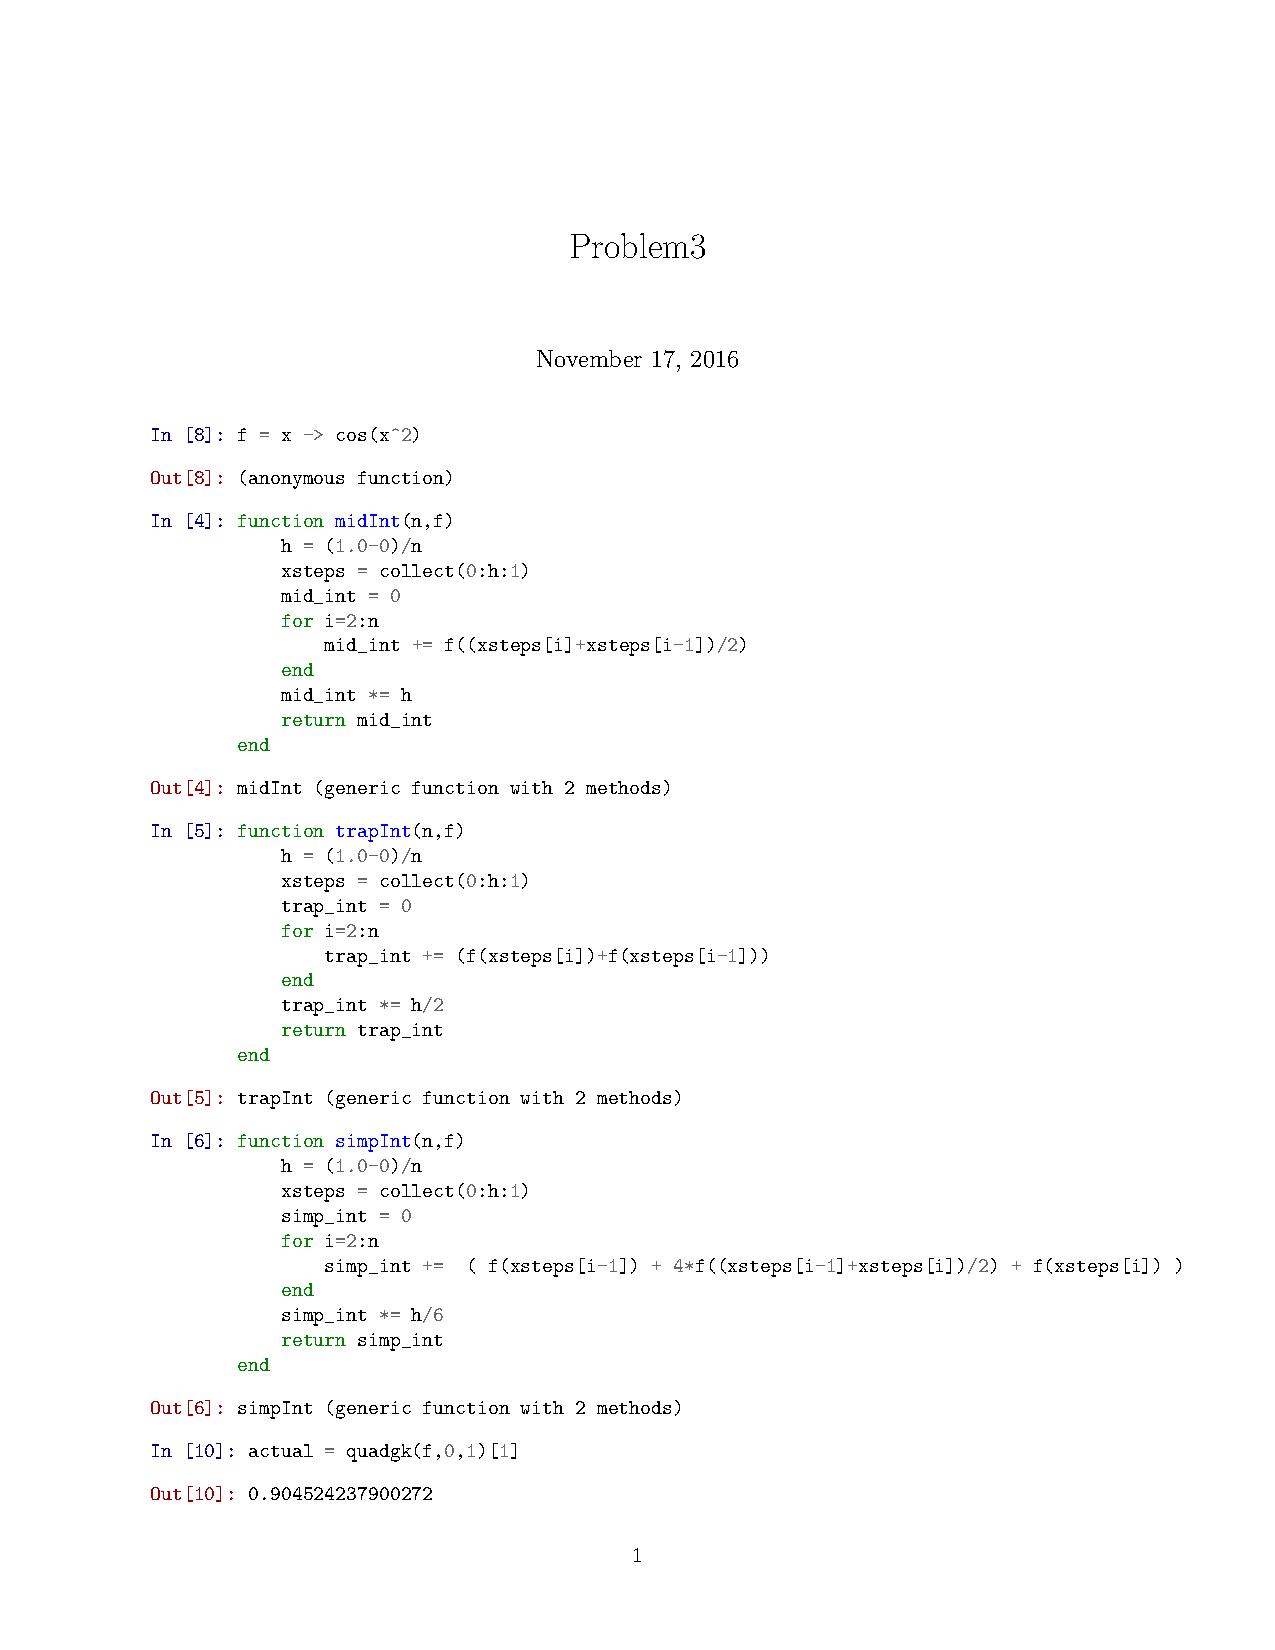
\includepdf[pages=-]{Problem3.pdf}
\subsection{Problem 4: Sleepless nights (20
points)}\label{problem-4-sleepless-nights-20-points}

\begin{enumerate}
\def\labelenumi{\arabic{enumi}.}
\tightlist
\item
  Chapter 11, Problem 3 (10 points)
\item
  Chapter 11, Problem 8 (10 points)
\end{enumerate}

\subsection{Problem 4 Solution}
\begin{enumerate}
\item
\[\frac{d}{dt} t^{3/2} =\frac{3}{2}t^{1/2} \]
Sub in $y=t^{3/2} \implies t=y^{2/3}$
\[ y'=\frac{3}{2}(y^{2/3})^(1/2) = \frac{3}{2}y^{1/3} \]
The reason this will not work is that it requires the value of y to change, and since it will be 0 Euler's method will not be able to properly evaluate the derivative. 

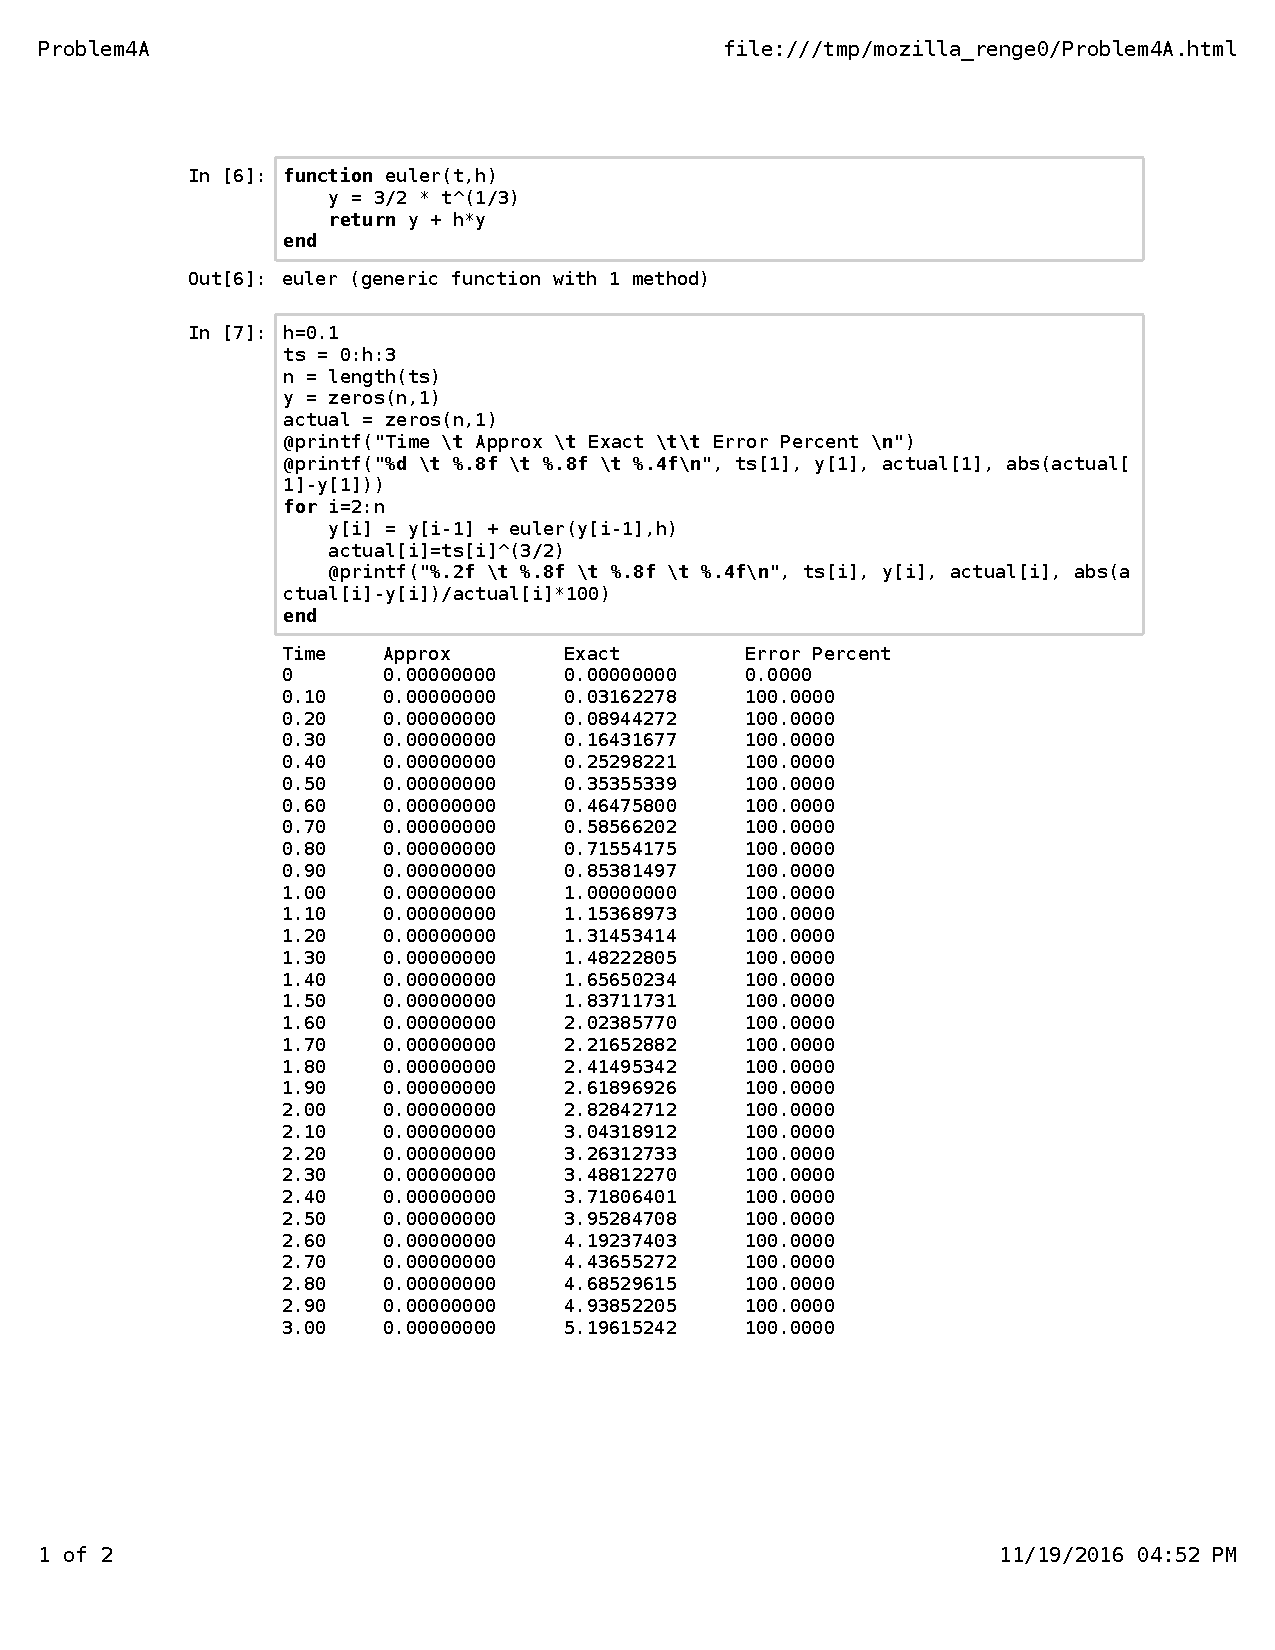
\includepdf[pages=-]{problem4A.pdf}
\item
	\begin{enumerate}
	\item
	The equations in 11.23 have Juliet's emotions brought down solely by Romeo's whose will rise as a result. This makes an elliptical orbit as observed. 
	\item
	\hfill \break
	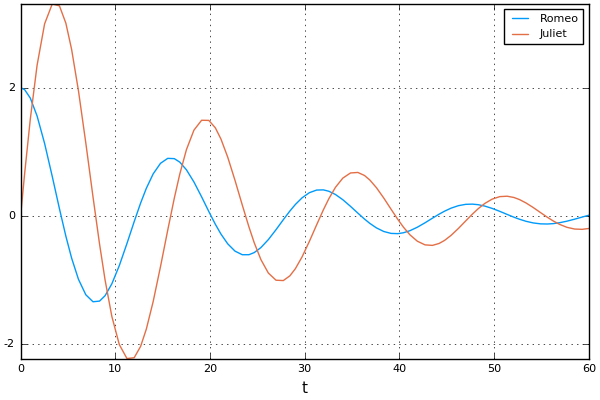
\includegraphics[width=\textwidth,keepaspectratio]{problem4B_1.png}
	\hfill \break
	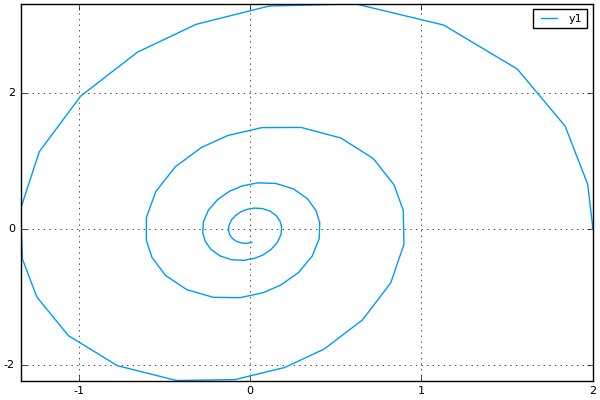
\includegraphics[width=\textwidth,keepaspectratio]{problem4B_2.png}
	\hfill \break
	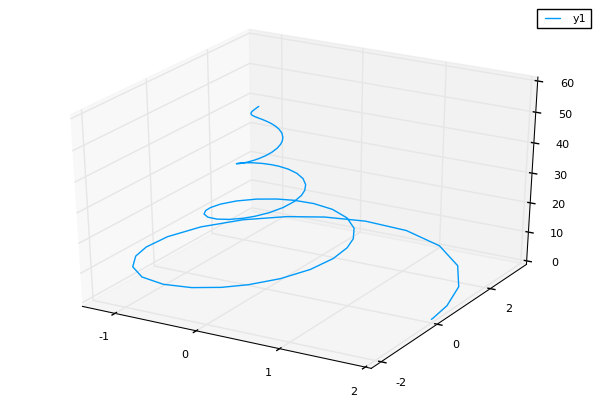
\includegraphics[width=\textwidth,keepaspectratio]{problem4B_3.png}
	
	\item
	Because Juliet's emotions are brought down by her own state, the emotions will converge towards indiference. 
	\end{enumerate}
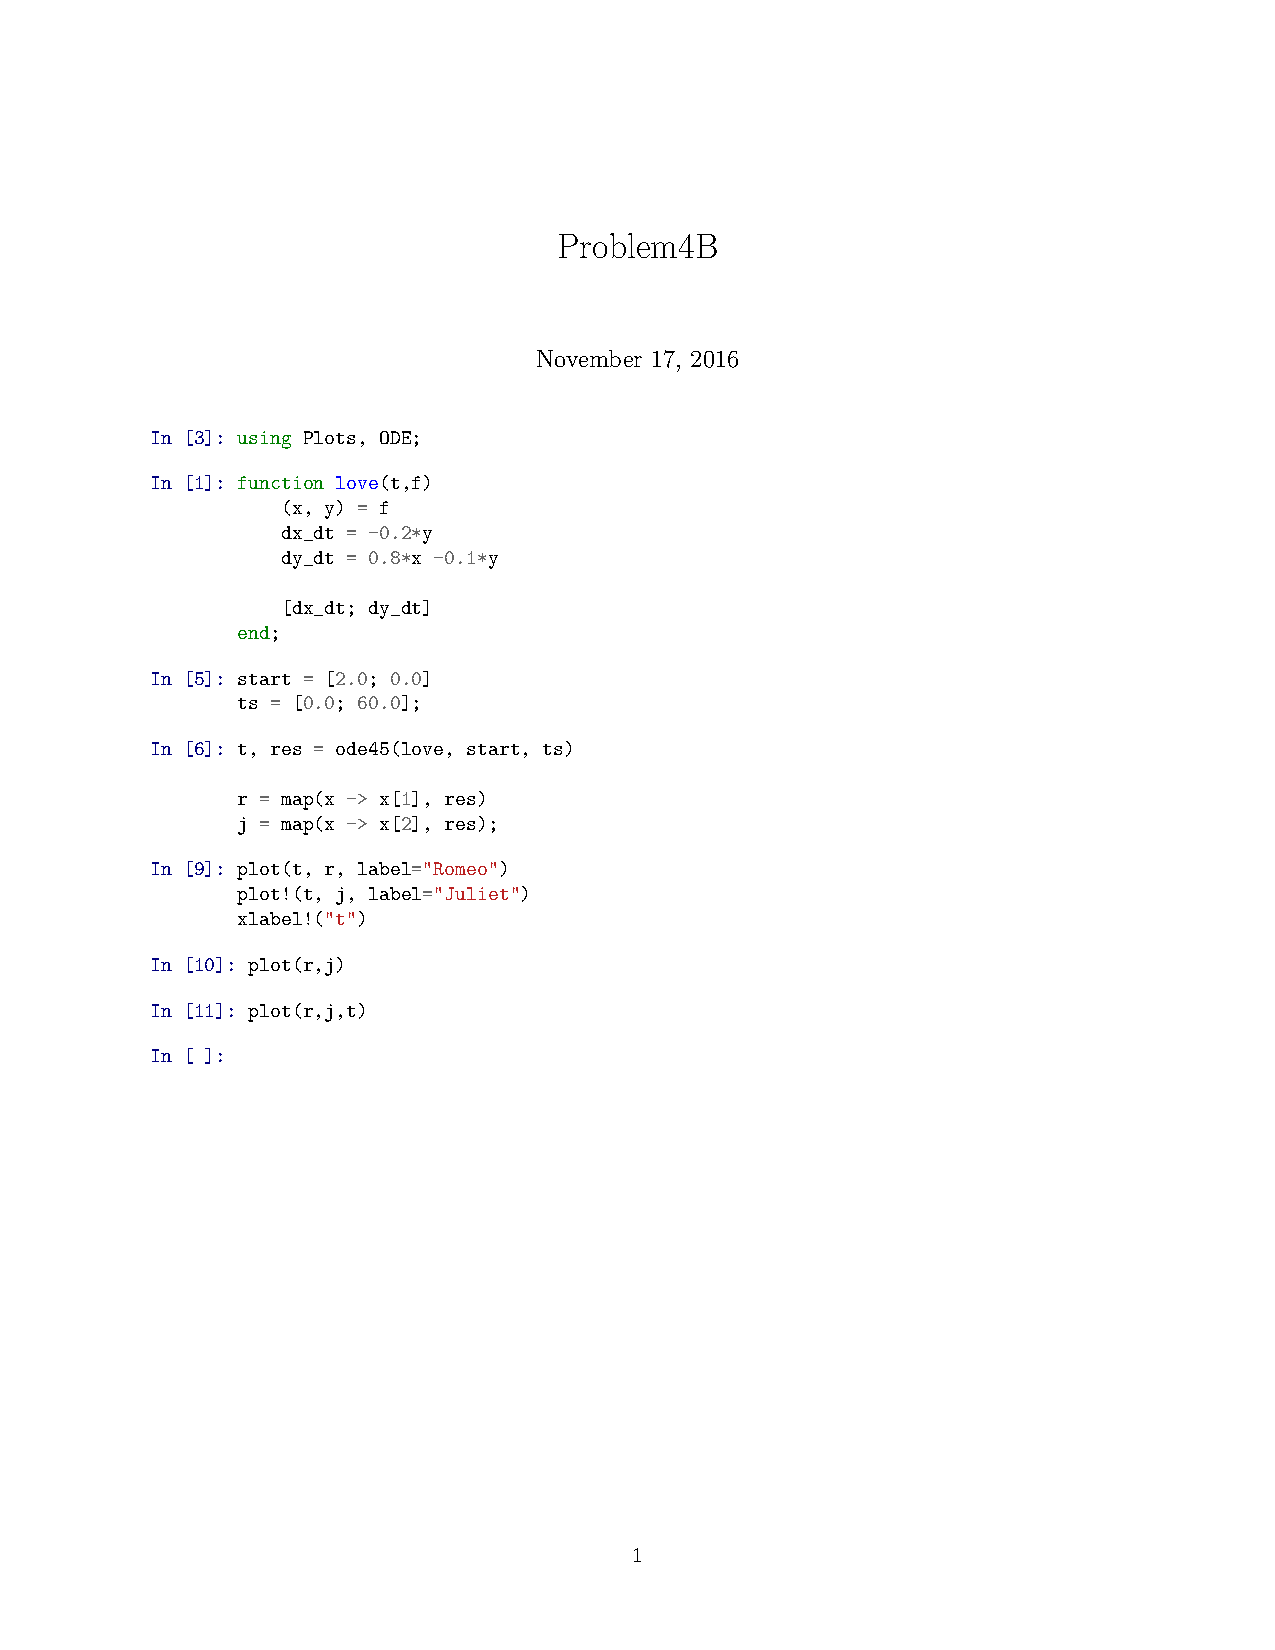
\includepdf[pages=-]{Problem4B.pdf}
\end{enumerate}

\subsection{Problem 5: A choice! (15
points)}\label{problem-5-a-choice-15-points}

Please choose your own adventure! You only need to do one of the
following problems.

\textbf{Theory} Chapter 11, Problem 11 (You will have to read in the
book about how to show multi-step methods are convergent.)

\textbf{Experiment} Chapter 11, Problem 14. Here, you should use the
version of 4th order Runge-Kutta in Section 11.2.5. Make sure you show
at least one illustration of the numerical problem described with small
\(w(0)\).

\subsection{Problem 5 Solution}
\begin{enumerate}
\item
\[x'(t) = z(t) \]
\[y'(t) = w(t)\]
\[z'(t) = \frac{-x}{(\sqrt{x^2+y^2})^3}\]
\[ w'(t) = \frac{-y}{(\sqrt{x^2+y^2})^3}\]
\item

\item
My method requires using the correct value of h which must be calculated based on the question. ODE45 already handles that, and is more accurate in portraying the real system. 
\end{enumerate}
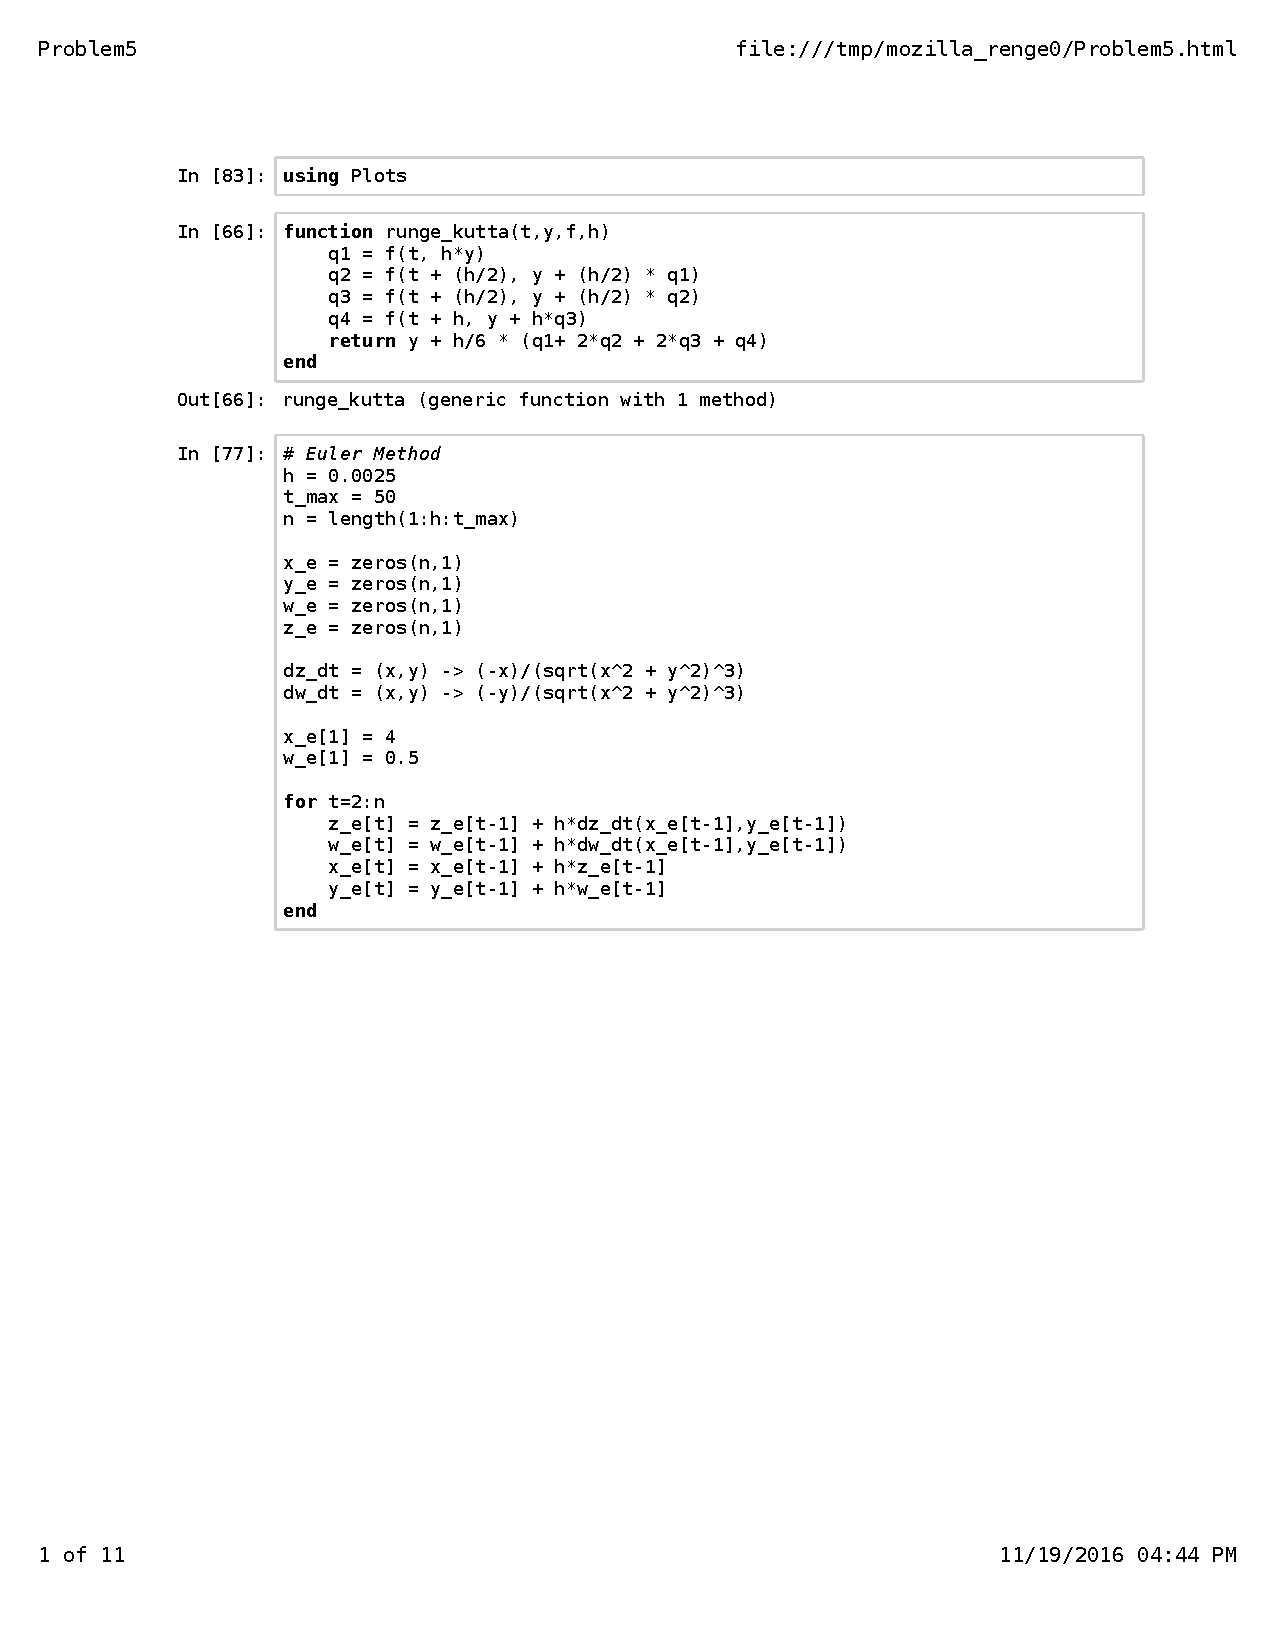
\includepdf[pages=-]{problem5.pdf}
\subsection{Problem 6: Look and explain! (10
points)}\label{problem-6-look-and-explain-10-points}

Take a look at the raptorchase code from the start of class. Go through
it an explain what each segment does! You may use as much or as little
granularity as you want.

\subsection{Problem 6}
At the start sets constants.  \\
Set max number of steps equal to 1000. For this that would mean each step takes place as 1/100th of a second \\
\textbf{Compute derivatives function }
\begin{enumerate}
\item 
The change of a human is given by the speed of the human and the x-direction and y-direction from angles
\item
From raptor 0 starting location, determines where the raptor's direction will be in order to face where the human is at that time step, then send the raptor in that direction by a unit of its velocity
\end{enumerate}
\textbf{Simulate Raptors}
This section will take initial positions, then will run forward Euler method on the raptop positions based on the behavior of the raptors and humans. Since the human will always move in a single direction, and the derivative is know it will be a straight line. The raptor's behavior depends on the position of the human, so this constantly shifting derivative and direction will look like a curve. The paths described are created by using an $h=0.01$ and the derivative function, and the position at time=t
\end{document}
